% ============================================================
%  深圳大学实验报告模板（SZU Experiment Report Template）
%  Project 1: NumPy re-implementation of the OpenCLIP ViT-B/32 image encoder
%  Compile with XeLaTeX.
% ============================================================

\documentclass[a4paper,12pt]{article}

% ----------------------------
% 中文与字体支持
% ----------------------------
\usepackage{fontspec}    % 字体支持
\usepackage{xeCJK}       % 中文字体支持
\setCJKmainfont{Noto Serif CJK SC} % 设置中文字体（Overleaf自带Noto字体）

% ----------------------------
% 页面设置与常用宏包
% ----------------------------
\usepackage{geometry}    % 页面边距控制
\geometry{left=1in, right=1in, top=1in, bottom=1in}

\usepackage{longtable}   % 支持长表格
\usepackage{graphicx}    % 插入图片
\usepackage{fancyhdr}    % 页眉页脚控制
\usepackage{tikz}        % 绘制框线等图形
\usetikzlibrary{calc}    % 坐标计算
\usepackage{verbatim}    % 显示代码块
\usepackage{float}       % 控制图片浮动位置（[H]参数）
\usepackage{xurl}        % 长链接可在任意位置断行，避免超出右边距
\usepackage{xcolor}      % 颜色（标红本人实现的部分）
\usepackage{listings}    % 带底纹与边框的代码块
\usepackage{enumitem}    % 收紧列表项间距，给正文留出页数余量

% ----------------------------
% 本人实现部分的标注配色
%   报告里凡是"本人写的代码"都用这套红色标注，与图 1 的红色图例对应
% ----------------------------
\definecolor{studentred}{HTML}{C0392B}    % 标注用的红色
\definecolor{studentbg}{HTML}{FDF1EC}     % 浅红底纹，保证黑字仍然清晰
\lstset{
  language=Python,
  basicstyle=\ttfamily\footnotesize,
  keywordstyle=\color{studentred}\bfseries,
  commentstyle=\color{black!55}\itshape,
  backgroundcolor=\color{studentbg},
  frame=single,
  framerule=0.9pt,
  rulecolor=\color{studentred},
  xleftmargin=3pt,
  xrightmargin=3pt,
  aboveskip=5pt,
  belowskip=5pt,
  showstringspaces=false,
  breaklines=true,
  keepspaces=true,
  columns=fullflexible,
}

% ----------------------------
% 排版微调
% ----------------------------
\setlength{\emergencystretch}{2em}   % 行内公式导致无法断行时允许适度拉伸
\makeatletter
\renewcommand\verbatim@font{\small\ttfamily}  % 代码块缩小一号，避免超出版心
\makeatother

% ----------------------------
% 页眉页脚设置
% ----------------------------
% \pagestyle{fancy}
\fancyhf{} % 清空默认页眉页脚
% \fancyhead[L]{深圳大学实验报告} % 左侧页眉文字
\fancyhead[C]{} % 中间空
\fancyhead[R]{} % 右侧空

% ============================================================
%                      文档开始
% ============================================================

\begin{document}

% ============================================================
% 封面页
% ============================================================
\begin{titlepage}
    \centering
    \vspace*{2cm}
    \Huge{\textbf{深 \ 圳 \ 大 \ 学 \ 实 验 报 告}}\\[1.5cm]
    
    {\Large\textbf{课程名称}\quad\underline{\makebox[8cm][c]{Python程序设计}}}\\[0.5cm]
{\Large
\noindent\makebox[3.2cm][l]{\textbf{项目名称}}
\underline{\makebox[8cm][c]{\large Project 1: NumPy Image Encoder}}}}\\[0.5cm]
{\Large
\noindent\makebox[3.2cm][l]{\textbf{学 \quad \quad 院}}
\underline{\makebox[8cm][c]{人工智能学院}}}\\[0.5cm]
{\Large
\noindent\makebox[3.2cm][l]{\textbf{专 \quad \quad 业}}
\underline{\makebox[8cm][c]{人工智能}}}\\[0.5cm]
{\Large
\noindent\makebox[3.2cm][l]{\textbf{指导教师}}
\underline{\makebox[8cm][c]{舒婷}}}\\[0.5cm]
{\Large
\noindent\makebox[3.2cm][l]{\textbf{报\hspace{0.92em}告\hspace{0.92em}人}}
\underline{\makebox[3cm][c]{古维滨}}
\hspace{0.5cm}
\textbf{学号}\hspace{0.18cm}
\underline{\makebox[3cm][c]{2025040079}}}\\[0.5cm]
{\Large
\noindent\makebox[3.2cm][l]{\textbf{实验时间}}
\underline{\makebox[8cm][c]{2026.11.17}}}\\[0.5cm]
{\Large
\noindent\makebox[3.2cm][l]{\textbf{提交时间}}
\underline{\makebox[8cm][c]{2026.11.22}}}\\[1.5cm]

    \vfill
    \Large{\textbf{教务处制}}
\end{titlepage}

\newpage

% ============================================================
% 正文部分
% ============================================================

\section{Objectives}

This report covers the NumPy rewrite of the image tower used by the final
project, the OpenCLIP ViT-B/32 vision encoder. Ten preprocessed
$224\times224$ RGB images and a fixed checkpoint of 152 visual tensors are
given; the encoder has to turn each image into one unit-length
512-dimensional vector, and the values have to match an FP32 reference
produced separately by PyTorch.

Three conditions had to be met. The six TODO groups are written with array
operations only, with no loop over samples, no framework call and no cached
reference values. Each stage has to land inside its published tolerance
($\mathrm{atol}=2\times10^{-4}$ for internal tokens, $2\times10^{-5}$ for the
final output token). And the public class interface has to stay as it is, so
that the file can be dropped next to \texttt{clip.py} without edits.


\section{Overview}

The encoder is a single feed-forward chain: no data-dependent branches and no training. Figure
\ref{fig:vit-arch} shows the five stages and which of them were written here and
which came with the starter code.

\begin{enumerate}[itemsep=2pt,topsep=3pt,parsep=0pt,leftmargin=2.4em]
    \item[Spot 1]: \textbf{patchify} cuts each image into a $7\times7$ grid of
    $32\times32$ patches and flattens them into 49 rows,
    $[B,3,224,224]\rightarrow[B,49,3072]$;
    \item[Spot 2]: \textbf{embed} projects patches to width 768 without bias,
    prepends one CLS row and adds learned positions, $\rightarrow[B,50,768]$;
    \item[Spot 3]: \textbf{twelve Transformer blocks}, each Norm, attention,
    residual, Norm, MLP, residual, with shapes unchanged throughout;
    \item[Spot 4]: \textbf{output head} keeps the CLS row, applies the
    post-Norm, projects $768\rightarrow512$ and scales to unit length;
    \item[Spot 5]: \textbf{preprocessing}, supplied: shortest-edge resize,
    centre crop and CLIP normalisation; every stage is then compared with the
    reference before the next one starts.
\end{enumerate}

% Figure
\begin{figure}[t]
    \centering
    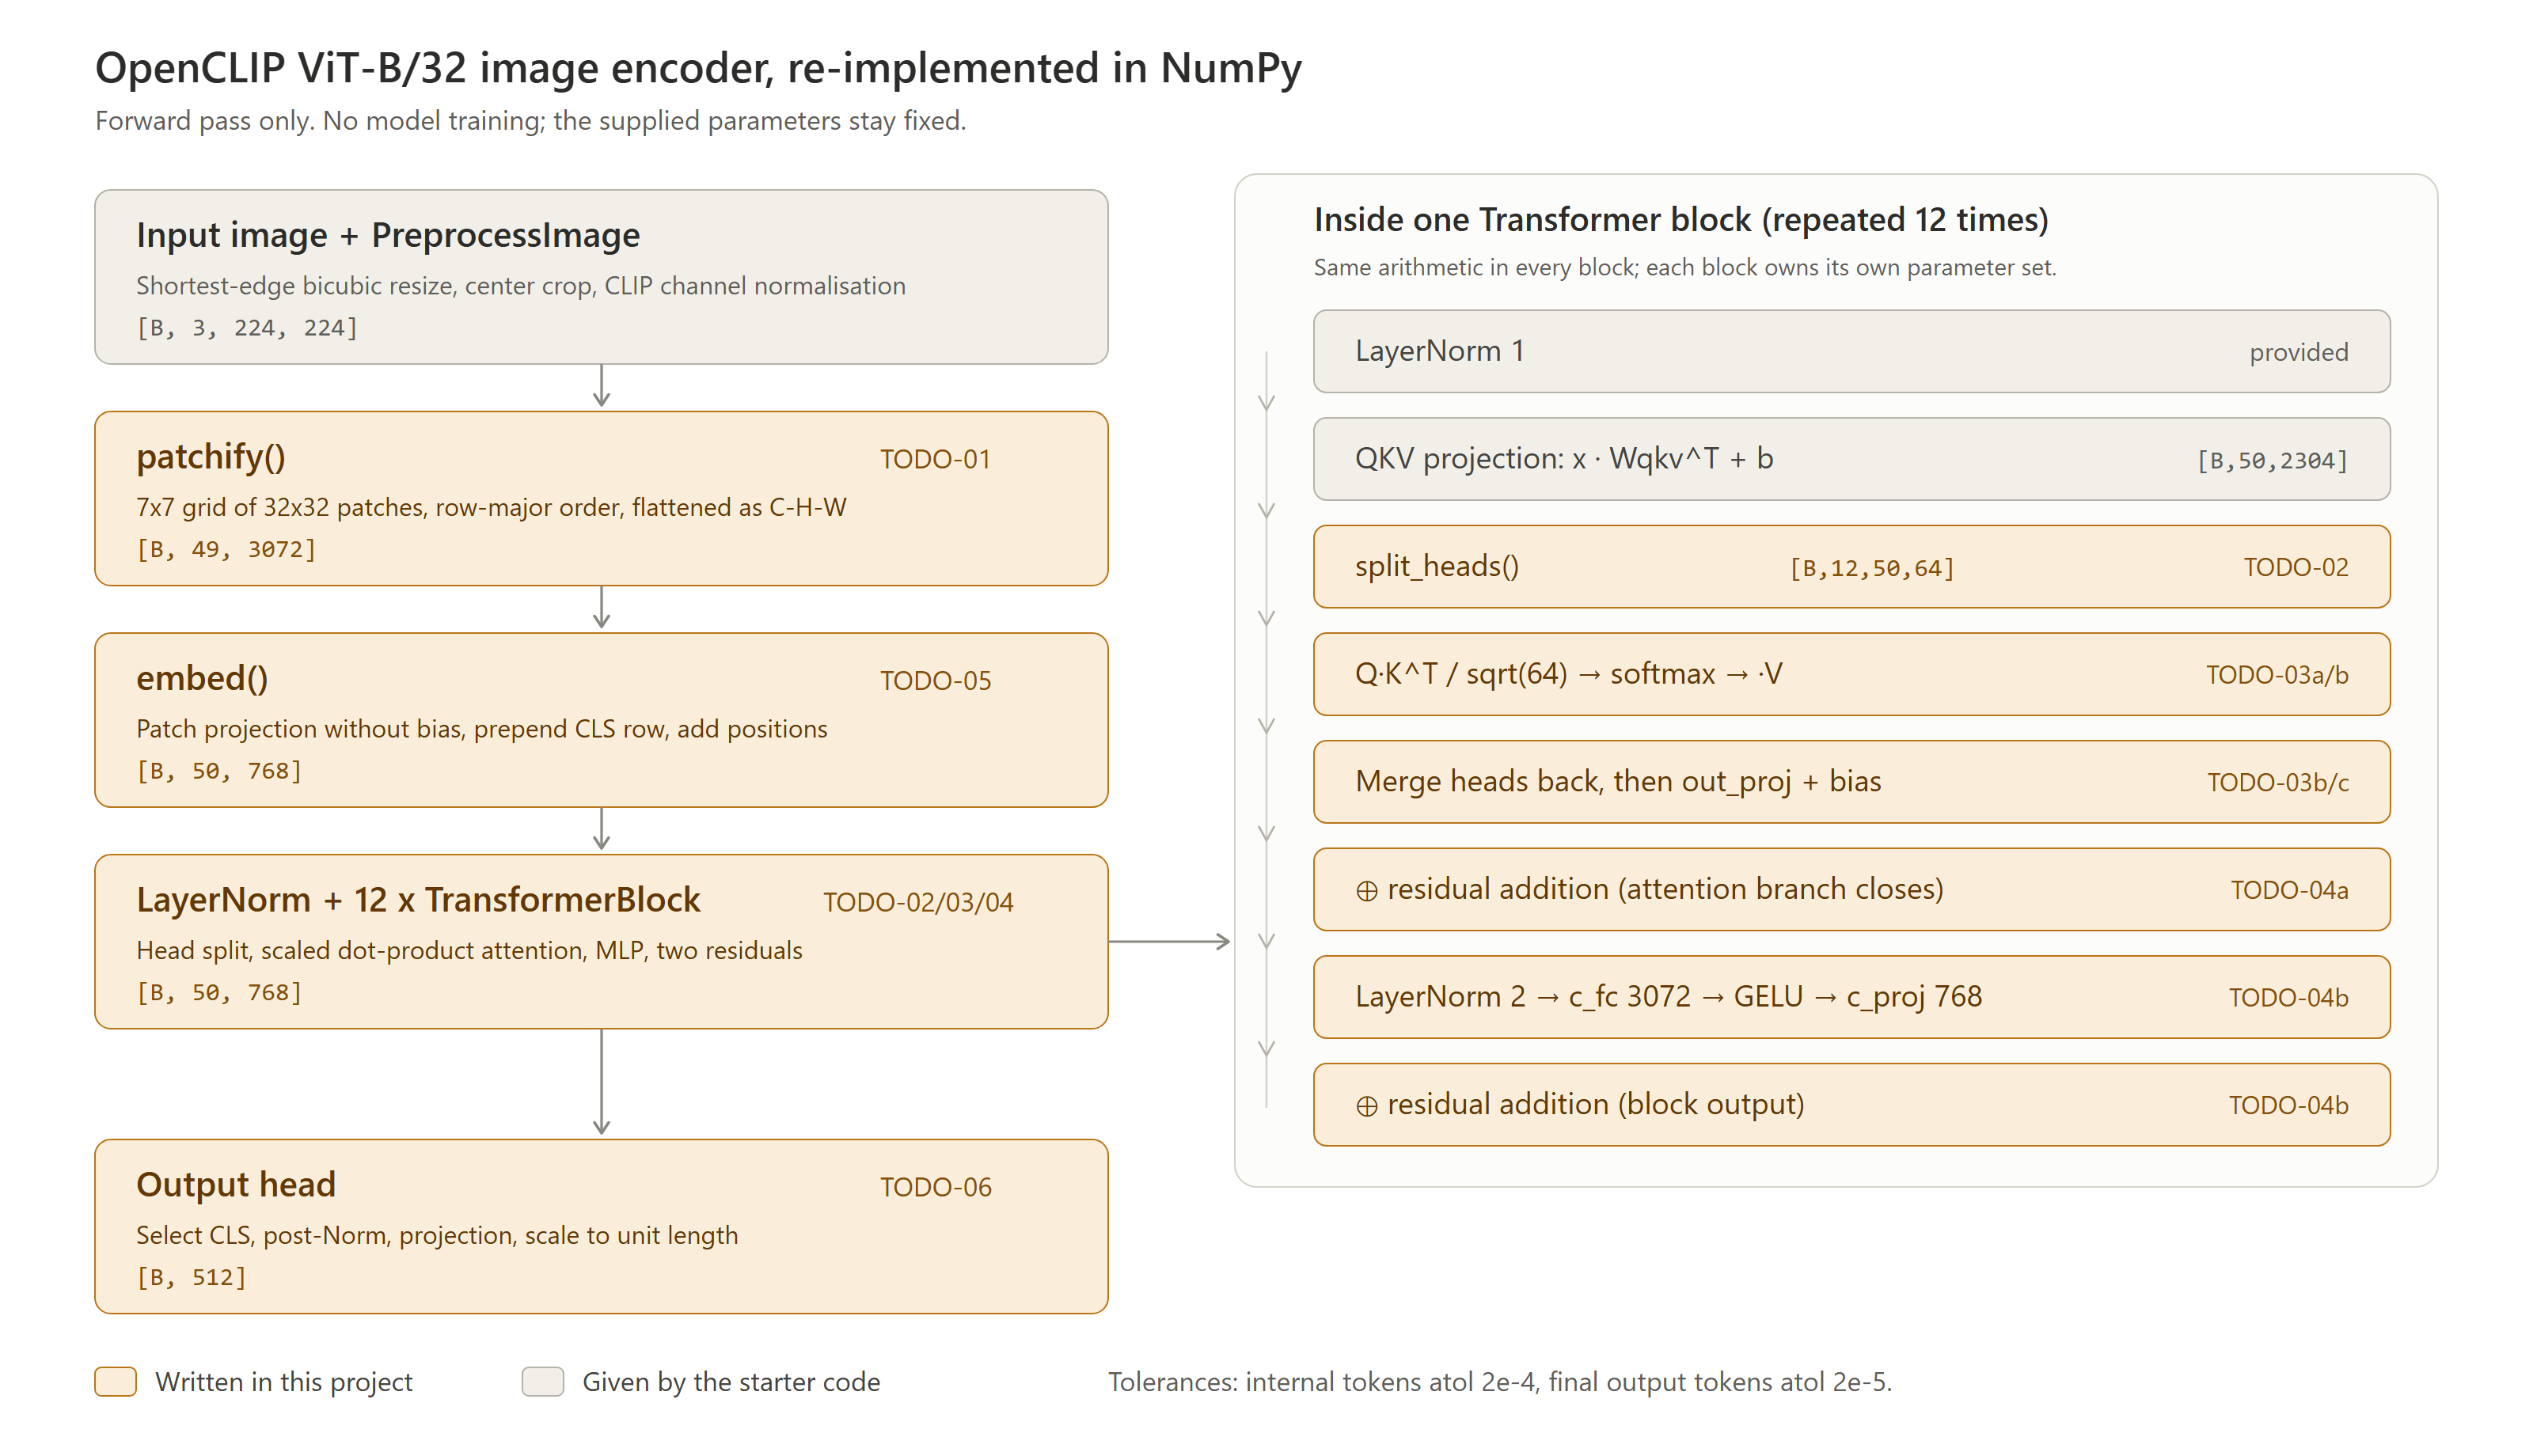
\includegraphics[width=0.98\linewidth]{figs/vit_overview.png}
    \caption{Left: the five stages of the encoder with the array shape carried
    between them. Right: the arithmetic inside one Transformer block. Red
    blocks are the parts written for this submission; grey blocks come with the
    starter code (preprocessing, LayerNorm, exact GELU, the softmax conversion
    and the unit-length helper).}
    \label{fig:vit-arch}
\end{figure}


\section{Implementations}

The work splits into five parts, written with indexing,
\texttt{reshape}/\texttt{transpose}, \texttt{@}, reductions and broadcasting,
plus \texttt{np.concatenate} and \texttt{np.tile} where a new axis has to be
filled in.

\begin{enumerate}[itemsep=2pt,topsep=3pt,parsep=0pt,leftmargin=2.4em]
    \item[Part 1] \textbf{Patches}: \texttt{patchify} (TODO-01),
    $[B,3,224,224]\rightarrow[B,49,3072]$;
    \item[Part 2] \textbf{Tokens}: \texttt{embed} (TODO-05),
    $\rightarrow[B,50,768]$;
    \item[Part 3] \textbf{Attention}: \texttt{split\_heads} (TODO-02) and
    the attention call (TODO-03), $\rightarrow[B,N,768]$;
    \item[Part 4] \textbf{Block}: \texttt{TransformerBlock.\_\_call\_\_}
    (TODO-04), $\rightarrow[B,N,768]$;
    \item[Part 5] \textbf{Output token}:
    \texttt{ImageEncoder.\_\_call\_\_} (TODO-06), $\rightarrow[B,512]$.
\end{enumerate}

The six TODO blocks behind these parts are excerpted below from
\texttt{image\_encoder.py} and framed in red, in the order the data flows rather
than the order of the numbers: embed (TODO-05) runs before attention (TODO-02)
because it creates the tokens attention reads. Each frame carries its TODO
number, the method it implements, and the shape before and after; the
\texttt{\# Given:} lines around them stay in the file, and TODO-03 starts at
\texttt{q/k/v} while TODO-06 starts at \texttt{tokens}.

\begin{lstlisting}[title={\color{studentred}\small \textbf{TODO-01}\;\textemdash\;\texttt{patchify}\enspace $[B,3,224,224]\rightarrow[B,49,3072]$}]
batch, channels, height, width = images.shape
patch_tokens = self.position.shape[0] - 1
grid = int(round(patch_tokens ** 0.5))
patch = height // grid
split = images.reshape(batch, channels, grid, patch, grid, patch)
ordered = split.transpose(0, 2, 4, 1, 3, 5)
return ordered.reshape(batch, grid * grid, channels * patch * patch)
\end{lstlisting}

\begin{lstlisting}[title={\color{studentred}\small \textbf{TODO-05}\;\textemdash\;\texttt{embed}\enspace $[B,49,3072]\rightarrow[B,50,768]$}]
projected = patches @ self.patch_weight.T
tokens = np.concatenate((cls, projected), axis=1)
return tokens + self.position
\end{lstlisting}

\begin{lstlisting}[title={\color{studentred}\small \textbf{TODO-02}\;\textemdash\;\texttt{split\_heads}\enspace $[B,N,768]\rightarrow[B,12,N,64]$}]
batch, tokens, width = x.shape
grouped = x.reshape(batch, tokens, self.heads, self.head_dim)
return grouped.transpose(0, 2, 1, 3)
\end{lstlisting}

\begin{lstlisting}[title={\color{studentred}\small \textbf{TODO-03}\;\textemdash\;\texttt{MultiHeadAttention.\_\_call\_\_}\enspace $[B,12,N,64]\rightarrow[B,N,768]$}]
scale = np.float32(np.sqrt(self.head_dim))
scores = (q @ k.transpose(0, 1, 3, 2)) / scale
context = coefficients @ v
merged = context.transpose(0, 2, 1, 3).reshape(
    x.shape[0], x.shape[1], self.width)
return merged @ self.out_weight.T + self.out_bias
\end{lstlisting}

\begin{lstlisting}[title={\color{studentred}\small \textbf{TODO-04}\;\textemdash\;\texttt{TransformerBlock.\_\_call\_\_}\enspace $[B,N,768]\rightarrow[B,N,768]$}]
residual = x + update
hidden = self.gelu(u @ self.fc1_weight.T + self.fc1_bias)
mlp_update = hidden @ self.fc2_weight.T + self.fc2_bias
return residual + mlp_update
\end{lstlisting}

\begin{lstlisting}[title={\color{studentred}\small \textbf{TODO-06}\;\textemdash\;\texttt{ImageEncoder.\_\_call\_\_}\enspace $[B,50,768]\rightarrow[B,512]$}]
cls = tokens[:, 0, :]
normalized = self.post_norm(cls)
output = normalized @ self.projection
return unit_vector(output)
\end{lstlisting}

Two of these frames cost me the most time. In TODO-01 the shape goes
$[B,3,7,32,7,32] \rightarrow [B,7,7,3,32,32] \rightarrow [B,49,3072]$: the first
\texttt{reshape} only regroups the axes, the \texttt{transpose} fixes their
order, and the second \texttt{reshape} merges the two axes the next stage
consumes. TODO-03 avoids \texttt{.T} because on a four-dimensional array it
reverses all four axes, so the three axes are named instead. TODO-06 is the easy one: \texttt{visual.proj}
is already $[in,out]$, so it is multiplied as it stands. Everything else in the
file is scaffolding and stays unmarked: the QKV projection, the causal mask, the
softmax conversion, the LayerNorms, the exact GELU, the twelve-block loop, the
weight arrays. Figure~\ref{fig:vit-arch} shows the same split in red and grey.


\section{Results}

Table~\ref{tab:errors} compares each stage against the supplied reference. Every
row passes. The final output token sits about 37 times inside its
tolerance.

\begin{table}[H]
\centering
\small
\caption{Staged numerical agreement with the independent FP32 reference
(ten images for the first and sixth rows, the first two images for the four
stages in between, a reordered and duplicated batch for the last row).}
\label{tab:errors}
\begin{tabular}{llrrrl}
\hline
Stage & Output shape & max abs error & mean abs error & atol & Result \\
\hline
preprocessing & (10, 3, 224, 224) & 0.0e+00 & 0.0e+00 & 2e-06 & PASS \\
patches       & (2, 49, 3072)      & 0.0e+00 & 0.0e+00 & 2e-04 & PASS \\
tokens        & (2, 50, 768)       & 4.005e-05 & 1.289e-06 & 2e-04 & PASS \\
block 0       & (2, 50, 768)       & 7.063e-06 & 3.250e-07 & 2e-04 & PASS \\
last tokens   & (2, 50, 768)       & 4.768e-05 & 2.696e-06 & 2e-04 & PASS \\
output token  & (10, 512)          & 5.439e-07 & 8.311e-08 & 2e-05 & PASS \\
batch order   & (3, 512)           & 4.619e-07 & 7.632e-08 & 2e-05 & PASS \\
\hline
\end{tabular}
\end{table}

I also ran two checks that \texttt{check.py} does not make. Tensors from
\texttt{run.py} come out as $(10,512)$ \texttt{float32}, all finite, every row
unit length to within $1.2\times10^{-7}$. Encoding the lecture cat photograph
together with a supplied image left that image's own row within
$5\times10^{-7}$ of its reference; a memorised answer would have drifted. The
last table row is already an order-and-duplicate test, but it uses
\texttt{allclose}; feeding the same image twice also gives bit-identical rows.

\noindent\textbf{Environment and commands.} All numbers in Table~1 come from one
machine: Windows 11 (x86-64), CPython 3.14.7, NumPy 2.5.5, Pillow 12.3.0, no
GPU. The staged comparison runs as \texttt{python check.py -{}-stage all}; the
export behind the shape and norm checks is
\texttt{python run.py -{}-output output\_tokens.npz}. Both load the checkpoint from
\texttt{weights/}; only \texttt{check.py} opens
\texttt{assets/reference\_outputs.npz}, and neither caches anything between
runs.


\section{Discussion}

\textbf{One shape change.} The first stage turns $[B,3,224,224]$ into
$[B,49,3072]$. Neither 49 nor 3072 appears anywhere in the input, so a plain
\texttt{reshape} cannot get there: 224 has to be split into $7\times32$ on both
spatial axes first, and the two grid axes then have to be moved in front of the
channel axis. \texttt{reshape} does the split, \texttt{transpose} does the move,
and the order handed to it is what fixes the rule ``left to right, then top to
bottom, and C-H-W inside a patch''. Drop the transpose and the array still has
the right shape, holding the right values in the wrong places. A shape check
cannot see that, which is why this stage is compared value by value.

\textbf{One bug fixed.} I copied \texttt{q @ k.T} from the lecture companion,
which works on a three-token, four-feature example. In the real model \texttt{k}
is $[B,12,50,64]$, so \texttt{.T} reversed all four axes into
$(64,50,12,B)$, and NumPy raised
\texttt{ValueError: matmul: Input operand 1 has a mismatch in its core
dimension 0}. The sizes in that message point at the head axis, which is not
where the mistake is. The fix is \texttt{k.transpose(0,1,3,2)}: it exchanges the
last two axes and leaves the image and head groups alone. What I took from it is
that \texttt{.T} stops meaning ``swap the last two axes'' past 2D, so the axes
have to be written out.

\textbf{Limitations.} The supplied GELU loops over scalar \texttt{math.erf}
calls, so one forward pass over ten images takes about a minute here. I left it alone,
because rewriting it would change the arithmetic that has to match the
reference. FP32 accumulation order also differs from PyTorch, which is why the
internal stages settle around $10^{-5}$ instead of exact zeros. The encoder
holds all twelve blocks and the whole batch in memory at once, fine for ten
images but not for a larger corpus.

\textbf{Next steps.} The next real step is the text tower, which can reuse
\texttt{TransformerBlock} as it stands, since the block already takes the
optional causal switch. Two smaller ones are a vectorised GELU, with a tolerance
study to show it still matches the reference, and a chunked path for batches too
large to hold.

\textbf{Contributions and assistance.} All six TODO groups in
\texttt{image\_encoder.py} were written for this submission; the scaffolding,
the checkpoint and the reference arrays are untouched. The red blocks in
Figure~\ref{fig:vit-arch} and the six red frames in Section~3 are the only work
claimed here; the rest of \texttt{image\_encoder.py} is scaffolding, and the
README, this report and \texttt{practice/numpy\_homework.py} are mine. I used an AI
assistant while working: it explained how the array shape moves between stages, proposed the
\texttt{transpose(0,2,4,1,3,5)} order in \texttt{patchify} and the
\texttt{transpose(0,2,1,3).reshape(...)} merge in attention, ran
\texttt{check.py} as I went, and helped with the \LaTeX. I checked both
expressions against the reference myself.

\noindent{\small Code, commit history and this report's source:
\url{https://github.com/GWB314/project1-numpy-student} (repository state as of
22 November 2026).}\par

\newpage

% ============================================================
% 批阅与成绩评定页
% ============================================================

% 绘制正文外框（包含批阅区域）
\begin{tikzpicture}[remember picture, overlay]
  \draw[thick] 
    ($(current page.north west)+(2cm,-3cm)$) 
    rectangle 
    ($(current page.south east)+(-2cm,3.5cm)$);
\end{tikzpicture}

\vspace{1cm}

% 批阅区
\noindent \textbf{指导教师批阅意见：}
\vspace{6cm}
\hfill

\vspace{1cm}

\noindent \textbf{成绩评定：}
\vspace{2cm}
\hfill

\vspace{1cm}

\noindent
\hfill
\textbf{指导教师签字：}\quad\quad\quad\quad\quad\\[0.5cm]

\hfill
\textbf{年}\quad\quad
\textbf{月}\quad\quad
\textbf{日}\quad

\vspace{1cm}

% 备注部分
\noindent \textbf{备注：}

% 框外的注释
\begin{tikzpicture}[remember picture, overlay]
  \node[
    anchor=north west,
    inner sep=0pt,
    text width=\dimexpr\paperwidth-4cm\relax
  ] at ($(current page.south west)+(2cm,3.1cm)$) {
    \begin{minipage}{\dimexpr\paperwidth-4cm\relax}
      \small
      \noindent
      \textbf{注：}\;1、报告内的项目或内容设置，可根据实际情况加以调整和补充。\\[0.2cm]
      \phantom{\textbf{注：}\;}2、教师批改学生实验报告时间应在学生提交实验报告时间后 10 日内。
    \end{minipage}
  };
\end{tikzpicture}

% ============================================================
%                      文档结束
% ============================================================

\end{document}

